\documentclass[hyperref={unicode,bookmarks=true, colorlinks=true,linkbordercolor=blue,urlbordercolor=blue,linkcolor=blue,urlcolor=blue,pdfborderstyle={/S/U/W 1}}]{beamer}


%\makeatletter
%	\Hy@AtBeginDocument{%
%	\def\@pdfborder{0 0 1}% Overrides border definition set with colorlinks=true
%	\def\@pdfborderstyle{/S/U/W 1}% Overrides border style set with colorlinks=true
%                                    % Hyperlink border style will be underline of width 1pt
%}
\makeatother


\usepackage[utf8]{inputenc}
\usepackage[russian]{babel}
\usepackage{tikz}
\usepackage{graphicx}
\usepackage[T1]{fontenc}
\usepackage[T2A]{fontenc}

\beamertemplatenavigationsymbolsempty
\usetheme{boxes}
\usecolortheme{beaver}
\usefonttheme{structurebold}
\useinnertheme{circles}
\usepackage{minted}
\usepackage{float}

\DeclareTextFontCommand{\emph}{\bfseries}
\definecolor{bgcode}{rgb}{0.90,0.90,0.90}

\author{Дмитрий Гурьянов}


\title{Объектно-ориентированное программирования на языке Java}

\begin{document}

\frame{\titlepage}

\section*{Содержание}
\begin{frame}
\tiny{\tableofcontents}
\end{frame}

\begin{frame}
	\frametitle{Определение ООП}

	\begin{large}
	\emph{Объектно-ориентированное программирование} -- парадигма программирования, в которой основными концепциями являются понятия объектов и классов. (©wikipedia)
	\end{large}
\end{frame}

\begin{frame}
	\frametitle{Объекты в реальном мире имеют состояние и поведение.}

	Объект: велосипед\\
	Состояние:
	\begin{itemize}
		\item{положение руля}
		\item{текущая передача}
		\item{скорость вращения педалей}
		\item{положение в пространстве}
	\end{itemize}
	Поведение:
	\begin{itemize}
		\item{сменить передачу}
		\item{повернуть руль}
		\item{узнать текущую скорость}
	\end{itemize}
\end{frame}

\begin{frame}[fragile]
	\frametitle{Объекты в программировании похожи на объекты из реального мира}

	\begin{columns}[c]
	\column{2.1in}
	\begin{large}
	Состояние -- набор полей, аналог полей структур в языке C.

	\medskip
	Поведение -- методы, аналог функций, применяемых к конкретному объекту.
	\end{large}
	\column{2.3in}
	\begin{minted}[bgcolor=bgcode]{java}
	class Bicycle {
	    /* fields */
	    float handlebarAngle;
	    int gear;
	    float cadence;
	    Vector pos;

	    /* methods */
	    void setGear(int gear);
	    void turn(float angle);
	    float getSpeed();
	}
	\end{minted}
	\end{columns}
\end{frame}

\begin{frame}
	\frametitle{Класс -- это тип объекта}
	\begin{large}
	В реальном мире много объектов с одинаковым набором свойств и поведением. Например много велосипедов одной модели.

	\medskip
	В программировании это называется классом. Каждый объект принадлежит какому-либо классу (является экземпляром этого класса).
	\end{large}
\end{frame}

\begin{frame}
	\frametitle{Свойства ООП}
	\begin{small}
	\begin{itemize}
		\item{Всё является объектом (в реальных языках часто это не так, например в Java есть небольшой набор простых типов данных, переменные этих типов не являются объектами).}
		\item{Вычисления осуществляются путём взаимодействия (обмена данными) между объектами, при котором один объект требует, чтобы другой объект выполнил некоторое действие. Объекты взаимодействуют, вызывая методы друг друга (аналоги функций в C)}
		\item{Каждый объект имеет независимую память, которая состоит из других объектов.}
		\item{Каждый объект является представителем класса, который выражает общие свойства объектов (таких, как целые числа или списки).}
		\item{В классе задаётся поведение (функциональность) объекта. Тем самым все объекты, которые являются экземплярами одного класса, могут выполнять одни и те же действия.}
	\end{itemize}
	\end{small}
\end{frame}

\begin{frame}[fragile]
	\frametitle{Сравним процедурное и объектно-ориентированное программирование}

	\begin{columns}[c]
	\column{2.1in}
	\emph{C-style}
	\medskip
	\begin{minted}[bgcolor=bgcode]{java}
	int fd;
	char buf[16];

	fd = open("file.txt");

	fseek(fd, 10);
	read(fd, buf, 16);

	close(fd);
	\end{minted}
	\column{2.1in}
	\emph{C++-style}
	\medskip
	\begin{minted}[bgcolor=bgcode]{java}
	File f;
	String s;

	f = new File("file.txt");

	f.fseek(10);
	s = f.read(16);

	delete f;
	\end{minted}
	\end{columns}
\end{frame}

\begin{frame}
	\frametitle{Java}

	\begin{Large}
	\emph{Java} — объектно-ориентированный язык программирования, разработанный компанией Sun Microsystems (в последующем приобретённой компанией Oracle). Дата официального выпуска — 23 мая 1995 года.
	\end{Large}
\end{frame}

\begin{frame}
	\frametitle{Java во многом отличается от C/C++}

	\begin{itemize}
		\item{Остутствуют возможности процедурного программирования (нет функций и структур в чистом виде)}
		\item{Остутствуют низкоуровневые возможности (работа с адресами скрыта, программист не должен делать никаких предположений о том, как передаются аргументы функций и.т.д.)}
		\item{Работа с памятью -- автоматическая, память объектов освобождается, когда не остается ссылок на них.}
		\item{Есть всего 8 простых типов данных, все остальные - классы}
		\item{Программа компилируется не в исполняемый файл, а в специальный байт-код, который затем может быть исполнен с помощью виртуальной машины java}
	\end{itemize}

\end{frame}


\begin{frame}[fragile]
	\frametitle{Hello World !}

	\begin{large}
	\emph{HelloWorldApp.java:}
	\begin{minted}[bgcolor=bgcode,gobble=0]{java}
	class HelloWorldApp {
	    public static void main(String[] args) {
	        System.out.println("Hello World!");
	    }
	}
	\end{minted}

	\emph{Компиляция:}
	\begin{minted}[bgcolor=bgcode,gobble=0]{bash}
	javac HelloWorldApp.java
	\end{minted}

	\emph{Запуск:}
	\begin{minted}[bgcolor=bgcode,gobble=0]{bash}
	java HelloWorldApp
	\end{minted}
	\end{large}

\end{frame}

\begin{frame}
	\frametitle{Простые типы данных}

	\begin{LARGE}
	\emph{byte, short, int, long, float, double, boolean, char}
	\end{LARGE}
\end{frame}

\begin{frame}[fragile]
	\frametitle{Посмотрим на пример описания и использования класса}
	\begin{minted}[bgcolor=bgcode,gobble=0,linenos=true,baselinestretch=0.7]{java}
	class Rectangle {
	    float x1, y1, x2, y2; 

	    Rectangle(float ix1, float iy1,
	              float ix2, float iy2) {
	        x1 = ix1; y1 = iy1;
	        x2 = ix2; y2 = iy2;
	    }   

	    float getSquare() {
	        return (x2 - x1) * (y2 - y1);
	    }   
	}

	class HelloWorldApp {
	    public static void main(String [] argc) {
	        Rectangle r = new Rectangle(1, 4, 7, 6);
	        float s = r.getSquare();
	        System.out.println(s);
	    }   
	}
	\end{minted}
\end{frame}

\begin{frame}[fragile]
	\frametitle{Использование объектов}

	\begin{minted}[bgcolor=bgcode,gobble=0,linenos=true]{java}
	class HelloWorldApp {
	    public static void main(String [] argc) {
	        Rectangle r1 = new Rectangle(1, 4, 7, 6);
	        Rectangle r2 = new Rectangle(0, 0, 5, 4);
	        float s = r1.getSquare();

	        System.out.println(s);
	        s = r2.getSquare();
	        System.out.println(s);
	    }
	}
	\end{minted}
\end{frame}


\begin{frame}[fragile]
	\frametitle{Статические поля и методы}

	\begin{large}
	Поля и методы, описанный с ключевым словом \emph{static} относятся не к объекту, а к классу.
	\end{large}

	\medskip
	\begin{minted}[bgcolor=bgcode,gobble=0,linenos=true,baselinestretch=1.0]{java}
	class Test {
	    static int x;
	    int y;

	    static void test1() {
	        System.out.println(x);
	    }

	    static void test2() {
	        System.out.println(y); /* error */
	    }
	}
	\end{minted}
\end{frame}

\begin{frame}[fragile]
	\frametitle{Статические поля и методы}
	\begin{minted}[bgcolor=bgcode,gobble=0,linenos=true,baselinestretch=1.0,firstnumber=13]{java}
	class HelloWorldApp {
	    public static void main(String [] argc) {
	        Test t1 = new Test();
	        Test t2 = new Test();
	        t1.x = 10;

	        System.out.println(t2.x);
	        t2.test1();

	        System.out.println(Test.x);
	        Test.test1();
	    }
	}
	\end{minted}

\end{frame}


\section{Введение в объектно-ориентированное программирование часть 2}
\subsection{Описание классов}
\begin{frame}[fragile]
	\frametitle{Конструкторы можно вызывать друг из друга}
	{\large Есть только одно ограничение -- вызов конструктора должен быть первый оператором.}

	\medskip
	\begin{minted}[bgcolor=bgcode,tabsize=4,linenos=true]{java}
		class Rectangle {
		    float x1, y1, x2, y2;

		    Rectangle(float ix1, float iy1,
		              float ix2, float iy2) {
		        x1 = ix1; y1 = iy1;
		        x2 = ix2; y2 = iy2;
		    }

		    Rectangle(float ix, float iy) {
		        Rectangle(0, 0, ix, iy);
		    }
		}
	\end{minted}

\end{frame}

\begin{frame}[fragile]
	\frametitle{Обычные методы тоже могут иметь одинаковые имена}

	\begin{large}
	\begin{minted}[bgcolor=bgcode,baselinestretch=0.8,linenos=true]{java}
		class Rectangle {
		    /* ... */
		    void scale(float sx, float sy) {
		        ix1 *= sx; ix2 *= sx;
		        iy1 *= sy; iy2 *= sy;
		    }

		    void scale(float s) {
		        ix1 *= s; ix2 *= s;
		        iy1 *= s; iy2 *= s;
		    }

		    /* better */
		    void scale(float s) {
		        scale(s, s);
		    }
		}
	\end{minted}
	\end{large}
\end{frame}

\begin{frame}[fragile]
	\frametitle{\textit{this} -- это ссылка на текущий объект}

	\begin{large}
	Используется для того, чтобы:
	\begin{itemize}
	\item{Передать ссылку на текущий объект в метод другого объекта}
	\item{Обратиться к полям, скрытым локальными переменными и параметрами методов}
	\end{itemize}
	\end{large}

	\begin{minted}[bgcolor=bgcode,baselinestretch=0.8,linenos=true]{java}
		class Rectangle {
		    float x1, y1, x2, y2;

		    Rectangle(float x1, float y1,
		            float x2, float y2) {
		        this.x1 = x1; this.y1 = y1;
		        this.x2 = x2; this.y2 = y2;
		    }
		
		    void testMethod(MyClass c) {
		        c.method(this);
		    }
		}
	\end{minted}
\end{frame}

\subsection{Массивы}
\begin{frame}[fragile]
	\frametitle{Массивы}

	\begin{Large}
	Объявление ссылки на массив:
	\begin{minted}[bgcolor=bgcode]{java}
	int arr[];
	Rectangle rects[];
	\end{minted}

	Создание массива:
	\begin{minted}[bgcolor=bgcode]{java}
	arr = new int[20];
	\end{minted}

	Создание массива объектов:
	\begin{minted}[bgcolor=bgcode]{java}
	rects = new Rectangle[2];
	rects[0] = new Rectangle(1, 2);
	rects[1] = new Rectangle(1, 3);
	\end{minted}
	\end{Large}
\end{frame}

\begin{frame}[fragile]
	\frametitle{Массивы}

	\begin{Large}
	Создание и заполнение массива:
	\begin{minted}[bgcolor=bgcode]{java}
	int arr[] = {1, 2, 3};
	Rectangle rects = { new Rectangle(1, 2),
	                    new Rectangle(1, 3)};
	\end{minted}

	Длина массива:
	\begin{minted}[bgcolor=bgcode]{java}
	System.out.println(rects.length);
	\end{minted}

	Работа с массивом:
	\begin{minted}[bgcolor=bgcode]{java}
	x = arr[0] + arr[1];
	for(i = 0; i < arr.length; i++)
	    System.out.println(arr[i]);
	\end{minted}

	\end{Large}
\end{frame}

\subsection{Строки}
\begin{frame}[fragile]
	\begin{Large}
	\frametitle{Строки в Java -- это объекты, а не массивы символов}

	Дополнительные возможности:
	\begin{itemize}
	\item{Создание как в языке С: \emph{\texttt{String s = "qwe";}}}
	\item{Доступен оператор \texttt{+}}
	\end{itemize}
	\medskip
	\begin{minted}[bgcolor=bgcode]{java}
	String s1 = "123";
	String s2 = "45";

	/* will print "12345" */
	System.out.println(s1 + s2);
	\end{minted}
	\end{Large}
\end{frame}

\begin{frame}[fragile]
	\frametitle{Полезные методы класса \textit{String}}

	\begin{large}
	Получить длину строки
	\begin{minted}[bgcolor=bgcode]{java}
	int length()
	\end{minted}

	Получить симовол в указанной позиции
	\begin{minted}[bgcolor=bgcode]{java}
	char charAt(int index)
	\end{minted}

	Сравнить строки (аналог функции \emph{strcmp} в С)
	\begin{minted}[bgcolor=bgcode]{java}
	int compareTo(String anotherString) 
	\end{minted}

	Сравнить строки (возвращает просто true или false)
	\begin{minted}[bgcolor=bgcode]{java}
	boolean equals(Object anObject)
	\end{minted}

	Сконвертировать в массив символов
	\begin{minted}[bgcolor=bgcode]{java}
	char[] toCharArray()
	\end{minted}
	\end{large}
\end{frame}

\begin{frame}[fragile]
	\frametitle{Полезные методы класса \textit{String}}

	\begin{large}
	Проверить, содержит ли данную последовательность символов
	\begin{minted}[bgcolor=bgcode]{java}
	boolean contains(CharSequence s)
	\end{minted}

	Разделить на части
	\begin{minted}[bgcolor=bgcode]{java}
	String[] split(String regex);
	\end{minted}

	Проверить, начинается ли строка с данной
	\begin{minted}[bgcolor=bgcode]{java}
	boolean startsWith(String prefix)
	\end{minted}

	\href{http://docs.oracle.com/javase/6/docs/api/java/lang/String.html}{документация по классу String}
	\end{large}
\end{frame}

\subsection{Работа с файлами}
\begin{frame}[fragile]
	\frametitle{Чтение байт из файла}

	\begin{Large}
	\begin{minted}[bgcolor=bgcode]{java}
	FileInputStream fis;
	byte [] buf = new byte[10];

	fis = new FileInputStream("1.txt");
	fis.read(buf);
	\end{minted}
	\end{Large}
\end{frame}

\begin{frame}[fragile]
	\frametitle{Чтение символов}

	\begin{columns}[c]
	\column{2.8in}
	\begin{minted}[bgcolor=bgcode]{java}
	FileInputStream fis;
	InputStreamReader is;
	char [] buf = new char[10];

	fis = new FileInputStream("1.txt");
	is = new InputStreamReader(
	                    is, "utf-8");

	is.read(buf);
	\end{minted}
	\column{1.7in}
	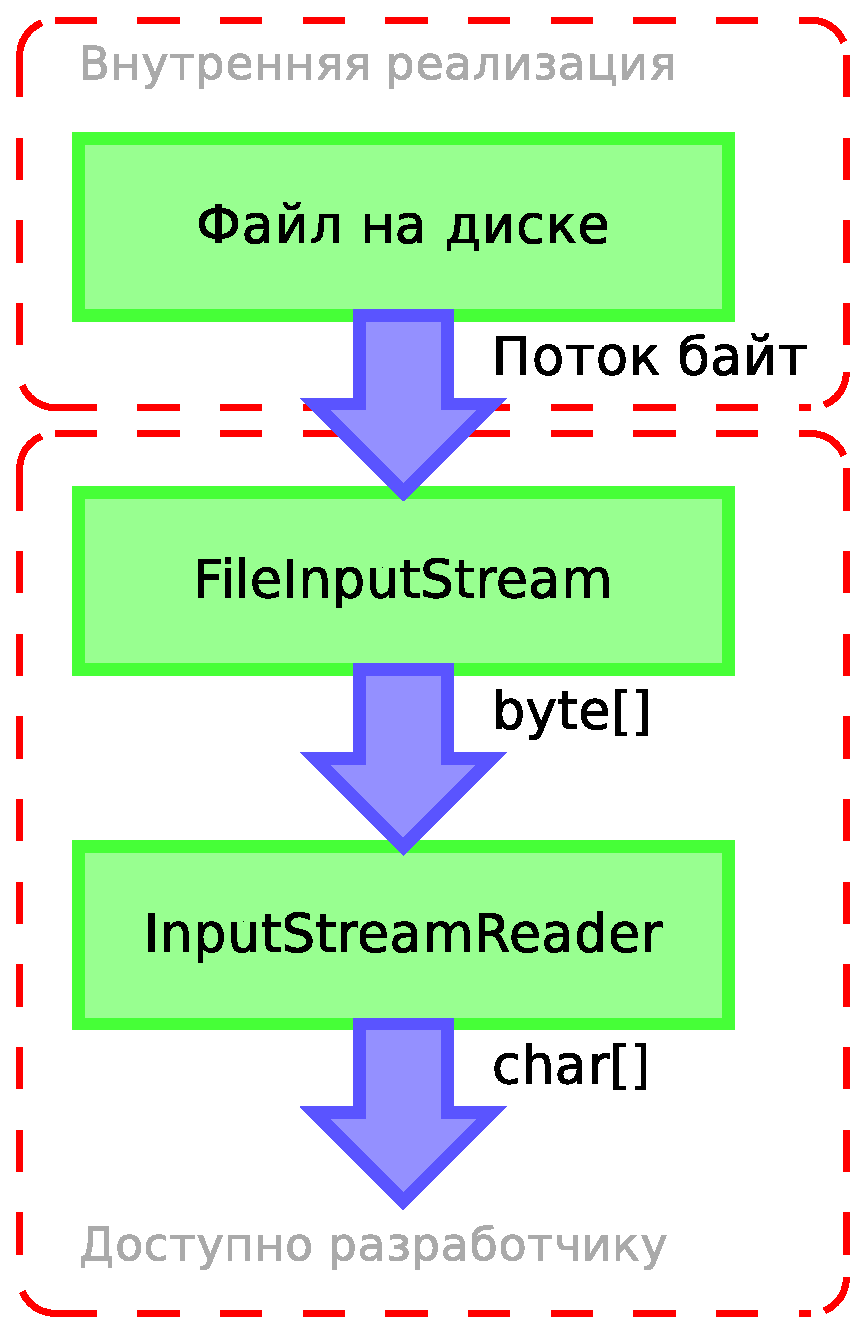
\includegraphics[width=1.75in]{lesson-3-Diagram1.eps}
	\end{columns}
\end{frame}

\begin{frame}[fragile]
	\frametitle{FileReader -- объединение FileInputStream и InputStreamReader для удобства}

	\begin{Large}
	
	\begin{minted}[bgcolor=bgcode]{java}
	FileReader fr;
	char [] buf = new char[10];

	fr = new FileReader("1.txt");
	fr.read(buf);
	\end{minted}
	\end{Large}
\end{frame}

\subsection{Задачи}
\begin{frame}[fragile]
	\frametitle{Задачи}

	\begin{enumerate}
		\begin{item}
			Написать программу для сортировки массива случайных чисел. Напечатать массив до и после сортировки.

			Дополнения:
			\begin{itemize}
				\item{Взять размер массива из параметра командной строки, если он не указан или указано более одного параметра - напечатать справку.}
				\item{Считать массив из параметров командной строки. Размер должен определяться из числа аргументов.}
			\end{itemize}
		\end{item}
		\begin{item}
			Найти все простые числа из диапазона, заданного в командной строке 
		\end{item}
		\begin{item}
			Вычислить заданную функцию от чисел из командной строки. Реализовать функции min, max, avg, sum.


			Пример использования:
			\begin{minted}[bgcolor=bgcode]{bash}
			~: java Calc max 12 65 123 5 12 4356 42
			4356
			\end{minted}

		\end{item}

	\end{enumerate}
\end{frame}

\subsection{Полезные ресурсы}
\begin{frame}
	\frametitle{Полезные ресурсы}

	\begin{itemize}
	\item{\href{http://docs.oracle.com/javase/6/docs/}{Официальная документация}}
	\item{\href{http://www.oracle.com/technetwork/java/javase/documentation/java-se-7-doc-download-435117.html}{Архив с официальной документацией}}
	\item{\href{http://docs.oracle.com/javase/tutorial/}{Java tutorials}}
	\item{\href{http://www.javable.com/tutorials/fesunov/}{Учебное пособие (на русском языке)}}
	\end{itemize}
\end{frame}



\section{Наследование}


\section{Пакеты и модификаторы доступа}
\subsection{Пакеты}

\begin{frame}[fragile]
	\frametitle{Библиотека Java — это сборник классов}

	\begin{Large}
	\begin{itemize}
	\item{Библиотеки нужны для того, чтобы использовать в своем проекте классы, написанные другими людьми или наоборот, написать классы, которые потом смогут использовать другие.}
	\item{Обычно проекты выполнены в виде библиотеки, в который каждый файл содержит один класс.}
	\end{itemize}
	\end{Large}
\end{frame}

\begin{frame}[fragile]
	\frametitle{Использование библиотек}

	\begin{large}
	Обычно физически библиотека это jar-файл (архив), но может быть и просто директорией. Для подключения библиотеки надо использовать параметр \emph{-cp} при компиляции и запуске или переменную окружения \emph{CLASSPATH}:
	\medskip

	\begin{minted}[bgcolor=bgcode]{bash}
	javac -cp /usr/share/java/protobuf.jar App.java
	javac -cp /home/student/mylib App.java
	
	export CLASSPATH=/home/student/mylib
	javac App.java
	\end{minted}
	\end{large}

	По-умолчанию подключена только системная библиотека Java.
\end{frame}

\begin{frame}[fragile]
	\frametitle{Библиотеки состоят из пакетов}

	Библиотека --- это очень большое хранилище классов, обычно она разделена на более мелкие --- пакеты.
	Например у нас есть следующая структура файлов на диске:
	\medskip
	\begin{columns}[c]
	\column{2.0in}
	\begin{verbatim}
mylib
   |-package1
       |-ClassA.java
       |-package2
          |-ClassB.java
	\end{verbatim}
	\medskip
	\begin{small}
	В файлах ClassA.java и ClassB.java должно быть указано имя пакета с помощью ключевого слова \emph{package}.
	\end{small}
	\column{2.45in}
	CLassA.java:
	\begin{minted}[bgcolor=bgcode]{java}
	package package1;

	class ClassA {
	};
	\end{minted}

	ClassB.java:
	\begin{minted}[bgcolor=bgcode]{java}
	package package1.package2;

	class ClassB {
	};
	\end{minted}
	\end{columns}
\end{frame}

\begin{frame}[fragile]
	\frametitle{Использование пакетов}
	\begin{large}
	Теперь мы можем подключить эту библиотеку и воспользоваться классами \emph{ClassA} и \emph{ClassB} из любого места:
	\medskip

	\begin{minted}[bgcolor=bgcode]{java}
	import package1.ClassA;
	import package1.package2.ClassB;

	class App {
	    ClassA a = new ClassA();
	    ClassB b = new ClassB();
	};
	\end{minted}

	Компиляция и запуск:
	\begin{minted}[bgcolor=bgcode]{bash}
	javac -cp /home/student/mylib App.java
	java -cp /home/student/mylib App
	\end{minted}
	\end{large}

\end{frame}

\begin{frame}[fragile]
	\frametitle{Различные варианты использования}

	\begin{large}
	Можно подключить один класс из пакета:
	\begin{minted}[bgcolor=bgcode]{java}
	import package1.ClassA;
	\end{minted}

	Все классы из пакета:
	\begin{minted}[bgcolor=bgcode]{java}
	import package1.*;
	\end{minted}

	Либо вообще не подключать с помощью \emph{import}, а каждый раз указывать полный путь:
	\begin{minted}[bgcolor=bgcode]{java}
	class App {
	    public static void main(String args[]) {
	        package1.ClassA a;
	        a = new package1.ClassA;
	    }
	}
	\end{minted}
	\end{large}
\end{frame}

\subsection{Модификаторы доступа}

\begin{frame}[fragile]
	\frametitle{Проблема с написанием классов для других}
	Допустим у нас был класс для описания линии:
	\begin{minted}[bgcolor=bgcode,linenos=true]{java}
	class Line {
	    int x1, y1, x2, y2;

	    Line(int x1, int y1, int x2, int y2) {
	        this.x1 = x1; this.y1 = y1;
	        this.x2 = x2; this.y2 = y2;
	    }

	    void draw(Graphics g) { ... };
	}
	\end{minted}

	Мы дали этот класс другу, который написал следующий код:
	\begin{minted}[bgcolor=bgcode,linenos=true]{java}
	Line l = new Line(10, 20, 30, 40);
	System.out.format("line: (%d-%d) - (%d-%d)",
	                  l.x1, l.y1, l.x2, l.y2);
	\end{minted}
\end{frame}

\begin{frame}[fragile]
	\frametitle{Проблема с написанием классов для других}
	Потом мы решили использовать новый класс Point для хранения координат:
	\begin{minted}[bgcolor=bgcode,linenos=true]{java}
	class Point {
	    int x, y;
	    Point(int x, int y) {
	        this.x = x; this.y = y
	    }
	}
	class Line {
	    Point p1, p2;
	    Line(int x1, int y1, int x2, int y2) {
	        p1 = new Point(x1, y1);
	        p2 = new Point(x2, y2);
	    }
	}
	\end{minted}

	После чего дали этот новый код другу. У него все сломалось.
\end{frame}

\begin{frame}[fragile]
	\frametitle{Что делать ?}
	\begin{Large}
	Надо описывать, что в нашем классе можно использовать и что нельзя. То, что можно использовать всем мы не должны менять ни в коем случае.\end{Large}
	
	\begin{small} (в этом случае придется обойти всех, кто воспользовался нашим классом, объяснить им, зачем мы сделали такое изменение, терпеливо выслушать нецензурную брань и уговорить их исправить свой код).\end{small}

	\medskip
	\begin{Large}
	Это можно сделать с помощью модификаторов доступа.
	\end{Large}
\end{frame}

\begin{frame}[fragile]
	\frametitle{Модификаторы доступа для классов}

	\begin{Large}
	\begin{itemize}
	\item{\emph{public} --- класс можно использовать везде}
	\item{\emph{без модификатора} - класс можно использовать только внутри пакета}
	\end{itemize}
	\end{Large}

	\begin{minted}[bgcolor=bgcode,linenos=true]{java}
	class Point {
	    ...
	};

	public class Line {
	    ....
	};
	\end{minted}

	\emph{public} классы обязательно должны быть описаны в файлах с таким же именем.
\end{frame}

\begin{frame}[fragile]
	\frametitle{Модификаторы доступа для членов класса}

	{\bf
	\begin{large}
	\begin{tabular}[b]{|l|c|c|c|c|}
	\hline
	&класс&пакет&подкласс&везде\\[2ex]
	\hline
	public&Y&Y&Y&Y\\[2ex]
	\hline
	protected&Y&Y&Y&X\\[2ex]
	\hline
	без модификатора&Y&Y&X&X\\[2ex]
	\hline
	private&Y&X&X&X\\[2ex]
	\hline
	\end{tabular}
	\end{large}
	}
\end{frame}

\begin{frame}[fragile]
	\frametitle{Пример}

	\emph{test/ClassA.java}:
	\begin{minted}[bgcolor=bgcode,linenos=true]{java}
	package test;
	class ClassA {
	    public int a;
	    int b;
	    protected int c;
	    private d;
	};
	\end{minted}

	\emph{test/ClassB.java}
	\begin{minted}[bgcolor=bgcode,linenos=true]{java}
	package test;
	class ClassB extends ClassA {
	    void method1() {
	        print(a + b); /* OK */
	        print(c); /* OK */
	        print(d); /* err */
	    };
	};
	\end{minted}
\end{frame}

\begin{frame}[fragile]
	\frametitle{Пример}
	\emph{Test.java}:
	\begin{minted}[bgcolor=bgcode,linenos=true]{java}
	import test.*;

	class Test {
	    void method2() {
	        ClassA x = new ClassA();
	        print(x.a); /* OK */
	        print(x.b); /* err */
	        print(x.c); /* err */
	        print(x.d); /* err */

	    }
	}
	\end{minted}

\end{frame}

\begin{frame}[fragile]
	\frametitle{Правила расстановки можификаторов доступа}
	\begin{enumerate}
	\begin{item}
	Поля делать \emph{private}. Eсли нужно получать доступ к полю извне --- написать методы для этого, например
	\begin{minted}[bgcolor=bgcode,linenos=true]{java}
	class ClassA {
	    private int x;
	    int getX() { return x; }
	    void setX(int x) { this.x = x; }
	}
	\end{minted}
	\end{item}
	\item{Если метод объявлен как \emph{public} --- нельзя менять его поведение, тип возвращаемого значения, аргументы. Также нельзя его удалять.}
	\item{Вспомогательные классы объявлять без модификатора.}

	\end{enumerate}
\end{frame}

\begin{frame}[fragile]
	\frametitle{Задача}
Написать класс для работы со стеком.
Сделать 3 класса: один класс, обекты которого будут храниться в стеке (например классы Point или Line из этого семинара), класс Node, в котором будет храниться указатель на элемент стека, и, например, указатели на предыдущий и следующий элементы. И класс Stack, который будет содержать методы push и pop.

Пример:

\begin{minted}[bgcolor=bgcode,linenos=true]{java}
Stack stack = new Stack();
Point p;

stack.push(new Point(1,2));
stack.push(new Point(2,3));

p = stack.pop();
print(p.getX());
\end{minted}

	
\end{frame}


\section{Пакеты и модификаторы доступа}
\subsection{Пакеты}

\begin{frame}[fragile]
	\frametitle{Библиотека Java — это сборник классов}

	\begin{Large}
	\begin{itemize}
	\item{Библиотеки нужны для того, чтобы использовать в своем проекте классы, написанные другими людьми или наоборот, написать классы, которые потом смогут использовать другие.}
	\item{Обычно проекты выполнены в виде библиотеки, в который каждый файл содержит один класс.}
	\end{itemize}
	\end{Large}
\end{frame}

\begin{frame}[fragile]
	\frametitle{Использование библиотек}

	\begin{large}
	Обычно физически библиотека это jar-файл (архив), но может быть и просто директорией. Для подключения библиотеки надо использовать параметр \emph{-cp} при компиляции и запуске или переменную окружения \emph{CLASSPATH}:
	\medskip

	\begin{minted}[bgcolor=bgcode]{bash}
	javac -cp /usr/share/java/protobuf.jar App.java
	javac -cp /home/student/mylib App.java
	
	export CLASSPATH=/home/student/mylib
	javac App.java
	\end{minted}
	\end{large}

	По-умолчанию подключена только системная библиотека Java.
\end{frame}

\begin{frame}[fragile]
	\frametitle{Библиотеки состоят из пакетов}

	Библиотека --- это очень большое хранилище классов, обычно она разделена на более мелкие --- пакеты.
	Например у нас есть следующая структура файлов на диске:
	\medskip
	\begin{columns}[c]
	\column{2.0in}
	\begin{verbatim}
mylib
   |-package1
       |-ClassA.java
       |-package2
          |-ClassB.java
	\end{verbatim}
	\medskip
	\begin{small}
	В файлах ClassA.java и ClassB.java должно быть указано имя пакета с помощью ключевого слова \emph{package}.
	\end{small}
	\column{2.45in}
	CLassA.java:
	\begin{minted}[bgcolor=bgcode]{java}
	package package1;

	class ClassA {
	};
	\end{minted}

	ClassB.java:
	\begin{minted}[bgcolor=bgcode]{java}
	package package1.package2;

	class ClassB {
	};
	\end{minted}
	\end{columns}
\end{frame}

\begin{frame}[fragile]
	\frametitle{Использование пакетов}
	\begin{large}
	Теперь мы можем подключить эту библиотеку и воспользоваться классами \emph{ClassA} и \emph{ClassB} из любого места:
	\medskip

	\begin{minted}[bgcolor=bgcode]{java}
	import package1.ClassA;
	import package1.package2.ClassB;

	class App {
	    ClassA a = new ClassA();
	    ClassB b = new ClassB();
	};
	\end{minted}

	Компиляция и запуск:
	\begin{minted}[bgcolor=bgcode]{bash}
	javac -cp /home/student/mylib App.java
	java -cp /home/student/mylib App
	\end{minted}
	\end{large}

\end{frame}

\begin{frame}[fragile]
	\frametitle{Различные варианты использования}

	\begin{large}
	Можно подключить один класс из пакета:
	\begin{minted}[bgcolor=bgcode]{java}
	import package1.ClassA;
	\end{minted}

	Все классы из пакета:
	\begin{minted}[bgcolor=bgcode]{java}
	import package1.*;
	\end{minted}

	Либо вообще не подключать с помощью \emph{import}, а каждый раз указывать полный путь:
	\begin{minted}[bgcolor=bgcode]{java}
	class App {
	    public static void main(String args[]) {
	        package1.ClassA a;
	        a = new package1.ClassA;
	    }
	}
	\end{minted}
	\end{large}
\end{frame}

\subsection{Модификаторы доступа}

\begin{frame}[fragile]
	\frametitle{Проблема с написанием классов для других}
	Допустим у нас был класс для описания линии:
	\begin{minted}[bgcolor=bgcode,linenos=true]{java}
	class Line {
	    int x1, y1, x2, y2;

	    Line(int x1, int y1, int x2, int y2) {
	        this.x1 = x1; this.y1 = y1;
	        this.x2 = x2; this.y2 = y2;
	    }

	    void draw(Graphics g) { ... };
	}
	\end{minted}

	Мы дали этот класс другу, который написал следующий код:
	\begin{minted}[bgcolor=bgcode,linenos=true]{java}
	Line l = new Line(10, 20, 30, 40);
	System.out.format("line: (%d-%d) - (%d-%d)",
	                  l.x1, l.y1, l.x2, l.y2);
	\end{minted}
\end{frame}

\begin{frame}[fragile]
	\frametitle{Проблема с написанием классов для других}
	Потом мы решили использовать новый класс Point для хранения координат:
	\begin{minted}[bgcolor=bgcode,linenos=true]{java}
	class Point {
	    int x, y;
	    Point(int x, int y) {
	        this.x = x; this.y = y
	    }
	}
	class Line {
	    Point p1, p2;
	    Line(int x1, int y1, int x2, int y2) {
	        p1 = new Point(x1, y1);
	        p2 = new Point(x2, y2);
	    }
	}
	\end{minted}

	После чего дали этот новый код другу. У него все сломалось.
\end{frame}

\begin{frame}[fragile]
	\frametitle{Что делать ?}
	\begin{Large}
	Надо описывать, что в нашем классе можно использовать и что нельзя. То, что можно использовать всем мы не должны менять ни в коем случае.\end{Large}
	
	\begin{small} (в этом случае придется обойти всех, кто воспользовался нашим классом, объяснить им, зачем мы сделали такое изменение, терпеливо выслушать нецензурную брань и уговорить их исправить свой код).\end{small}

	\medskip
	\begin{Large}
	Это можно сделать с помощью модификаторов доступа.
	\end{Large}
\end{frame}

\begin{frame}[fragile]
	\frametitle{Модификаторы доступа для классов}

	\begin{Large}
	\begin{itemize}
	\item{\emph{public} --- класс можно использовать везде}
	\item{\emph{без модификатора} - класс можно использовать только внутри пакета}
	\end{itemize}
	\end{Large}

	\begin{minted}[bgcolor=bgcode,linenos=true]{java}
	class Point {
	    ...
	};

	public class Line {
	    ....
	};
	\end{minted}

	\emph{public} классы обязательно должны быть описаны в файлах с таким же именем.
\end{frame}

\begin{frame}[fragile]
	\frametitle{Модификаторы доступа для членов класса}

	{\bf
	\begin{large}
	\begin{tabular}[b]{|l|c|c|c|c|}
	\hline
	&класс&пакет&подкласс&везде\\[2ex]
	\hline
	public&Y&Y&Y&Y\\[2ex]
	\hline
	protected&Y&Y&Y&X\\[2ex]
	\hline
	без модификатора&Y&Y&X&X\\[2ex]
	\hline
	private&Y&X&X&X\\[2ex]
	\hline
	\end{tabular}
	\end{large}
	}
\end{frame}

\begin{frame}[fragile]
	\frametitle{Пример}

	\emph{test/ClassA.java}:
	\begin{minted}[bgcolor=bgcode,linenos=true]{java}
	package test;
	class ClassA {
	    public int a;
	    int b;
	    protected int c;
	    private d;
	};
	\end{minted}

	\emph{test/ClassB.java}
	\begin{minted}[bgcolor=bgcode,linenos=true]{java}
	package test;
	class ClassB extends ClassA {
	    void method1() {
	        print(a + b); /* OK */
	        print(c); /* OK */
	        print(d); /* err */
	    };
	};
	\end{minted}
\end{frame}

\begin{frame}[fragile]
	\frametitle{Пример}
	\emph{Test.java}:
	\begin{minted}[bgcolor=bgcode,linenos=true]{java}
	import test.*;

	class Test {
	    void method2() {
	        ClassA x = new ClassA();
	        print(x.a); /* OK */
	        print(x.b); /* err */
	        print(x.c); /* err */
	        print(x.d); /* err */

	    }
	}
	\end{minted}

\end{frame}

\begin{frame}[fragile]
	\frametitle{Правила расстановки можификаторов доступа}
	\begin{enumerate}
	\begin{item}
	Поля делать \emph{private}. Eсли нужно получать доступ к полю извне --- написать методы для этого, например
	\begin{minted}[bgcolor=bgcode,linenos=true]{java}
	class ClassA {
	    private int x;
	    int getX() { return x; }
	    void setX(int x) { this.x = x; }
	}
	\end{minted}
	\end{item}
	\item{Если метод объявлен как \emph{public} --- нельзя менять его поведение, тип возвращаемого значения, аргументы. Также нельзя его удалять.}
	\item{Вспомогательные классы объявлять без модификатора.}

	\end{enumerate}
\end{frame}

\begin{frame}[fragile]
	\frametitle{Задача}
Написать класс для работы со стеком.
Сделать 3 класса: один класс, обекты которого будут храниться в стеке (например классы Point или Line из этого семинара), класс Node, в котором будет храниться указатель на элемент стека, и, например, указатели на предыдущий и следующий элементы. И класс Stack, который будет содержать методы push и pop.

Пример:

\begin{minted}[bgcolor=bgcode,linenos=true]{java}
Stack stack = new Stack();
Point p;

stack.push(new Point(1,2));
stack.push(new Point(2,3));

p = stack.pop();
print(p.getX());
\end{minted}

	
\end{frame}

\end{document}

